\documentclass[a4paper,article,12pt,oneside]{memoir}
\OnehalfSpacing%
\setlrmarginsandblock{3cm}{2cm}{*}
\setulmarginsandblock{3cm}{2cm}{*}
\checkandfixthelayout%

\usepackage{csquotes}
\usepackage[english,german,french,main=brazil]{babel}
\usepackage{fontspec}
\setmainfont{Brill}
\setmonofont[Scale=0.70]{Noto Sans Mono}
\usepackage{hyperref}
\usepackage[table,x11names]{xcolor}
\usepackage{linguex}
\usepackage{paralist}
\usepackage[normalem]{ulem}
\usepackage{indentfirst}
\usepackage{graphicx}

\setlength{\footmarksep}{0em}
\setlength{\footmarkwidth}{0em}
\setlength{\thanksmarksep}{0em}
\setlength{\thanksmarkwidth}{0em}
\pagestyle{simple}

\newcommand{\agradecimentos}{Este projeto foi financiado pela FAPESP por meio dos processos de número \texttt{2017/23334-2}, \texttt{2019/18473-9} e \texttt{2021/06027-4}. Este \emph{paper} resulta do trabalho final da disciplina \texttt{FLL5133} \emph{Linguística Computacional}. Agradeço a Marcos Lopes (USP), Martina Rodda (\foreignlanguage{english}{Univerisity of Oxford}) e Richard McElreath (\foreignlanguage{german}{Max-Planck-Institut für evolutionäre Anthropologie}) pelas discussões sobre os métodos e a interpretação dos dados. Quaisquer falhas são, naturalmente, da minha parte. Todos os dados e o código utilizado neste trabalho estão disponíveis em~\url{https://github.com/caiogeraldes/2023sbec}.}

\title{Ser necessário fazer e ordenar fazer:\\{\Large classificadores gêneros literários por meio de classes verbais do grego}}
\author{Caio B. A. Geraldes\thanks{\agradecimentos}\vspace{5pt}\\{\normalsize{}FFLCH--USP}\\{\normalsize\url{caio.geraldes@usp.br}}}


\renewcommand{\figureautorefname}{Figura}
\renewcommand{\tableautorefname}{Tabela}
\renewcommand{\sectionautorefname}{seção}

\definecolor{green}{RGB}{16,89,66} % rgb(16,89,66)
\definecolor{orange}{RGB}{217,95,2} % rgb(217,95,2)

\hypersetup{colorlinks=true, linkcolor=green, citecolor=green, filecolor=magenta, urlcolor=green, bookmarksdepth=4}

\usepackage[backend=biber,
	style=abnt,
	pretty,
	repeatfields,
	noslsn,
	natbib,
	extrayear,
]{biblatex}
\addbibresource{./bibliografia/biblio.bib}


\begin{document}

\maketitle%

\begin{abstract}
	\noindent Neste trabalho, utilizo métodos de processamento de linguagem natural e quantitativos para produzir evidência formal para esta hipótese de distribuição de classes verbais entre gêneros literários. Utiliza-se o modelo Naïve-Bayes de classificador para verificar se a seleção lexical de verbos é suficientemente diferente entre os gêneros historiográfico e filosófico e são extraídos os coeficientes de peso dos verbos de interesse na classificação dos gêneros para observar se as classes verbais semânticas possuem efeito significativo na classificação. O resultado positivo permite considerar a associação entre autoria e gênero e atração de caso espúria e causada pela associação entre classe verbal e gênero literário.\vspace{4pt}\\
	\noindent \textbf{Palavras-chave:} semântica; gêneros literários; métodos quantitativos; grego antigo
\end{abstract}

\chapter{Introdução}

Em trabalhos anteriores~\cite{Geraldes2020,Geraldes2021}, mostrei que atração de caso infinitiva em grego clássico, isto é, a concordância de caso entre objeto indireto da matriz e predicado secundário de uma oração infinitiva (exemplificadas em~\ref{gloss:attrac}, sendo~\ref{elthonta} um exemplo sem a concordância de caso e~\ref{elthonti} com), está correlacionada com os seguintes fatores:
\begin{inparaenum}[(a)]
	\item distância entre controlador e alvo; quanto menor, mais frequente;
	\item classe de verbo infinitivo; a atração ocorrendo preferencialmente com cópulas;
	\item classe do verbo matriz, preferencialmente com verbos com sentido modal\slash{}deôntico;
	\item autoria, sendo a atração mais frequente em Platão do que em Xenofonte e praticamente inexistente em Heródoto.
\end{inparaenum}

\ex.\label{gloss:attrac}\ag.\label{elthonta}symbọːléw-ẹː \uwave{tɔ̂ːj Ksenopʰɔ̂ːnti} \uline{eltʰónt-ɑ} {ẹːs delpʰọːs} ɑnɑkojnoɔ̂ːs-ɑj {tɔ̂ːj tʰeɔ̂ːj} {peri tɛ̂ːs porẹ́ːɑs}\\
aconselha-\textsc{3sg} X.\textsc{dat.sg.m} indo-\textsc{acc.sg.m} para-Delfos interrogar.\textsc{inf} o-deus.\textsc{dat.sg} sobre-a-viagem\\
Ele aconselha Xenofonte ir a Delfos interrogar o deus sobre a viagem. (Xen. Anab. 3.1.5)
\bg.\label{elthonti}ɑpʰɛ̂ːk-e \uwave{moj} \uline{eltʰónt-i} {pros hymɑ̂s} légẹːn tɑlɛːtʰɛ̂ː\\
permitiu-\textsc{3sg} \textsc{pron{(1sg.dat.sg)}} indo-\textsc{dat.sg.m} frente-a-vós dizer.\textsc{inf} a-verdade-\textsc{acc.pl.n}\\
Ele me permitiu ir frente a vós [e\slash{}para] dizer a verdade.\\(Xen. Hell. 6.1.13)\footnote{Os exemplos utilizados foram retirados das edições disponibilizadas no TLG~\cite{tlg}. Para garantir o cotejo dos exemplos por público não especializado, realizei a transliteração automaticamente utilizando o pacote \texttt{cltk}~\cite{cltk}, o qual segue a reconstrução fonológica apresentada em~\textcite{Probert2010}.}

Os dois fatores com maior correlação são a classe do verbo principal~\footnote{Pearsons's $\chi^2 = 36.370 (1) p = 1.6-09$.} e a autoria.~\footnote{Pearson’s $\chi² = 16.506 (2), p =2.6e-04$.}
Uma vez que é impossível comparar resultados de testes estatísticos e valores $p$, não se pode deduzir a partir deles qual fator é mais determinante para a ocorrência da atração, sendo assim necessário estabelecer, a partir da teoria, um modelo causal gerativo -- não confundir com modelo \emph{sintático} gerativo.

Antes de apresentar o modelo causal que defendo, são necessárias algumas explicações sobre as ``classes verbais'' estatisticamente correlacionadas com a atração.
Os verbos que permitem a atração de caso regem um objeto em caso oblíquo (dativo ou genitivo) e uma oração infinitiva, organizando-se em três classes:
\begin{compactenum}
	\item verbos pessoais com a semântica de `\emph{ordenar}\slash{}\emph{pedir} \slash{}\emph{aconselhar}\slash{}etc. [a alguém] [fazer algo]' (e.g. παραγγέλλω, δέομαι e συμβουλεύω);
	\item a forma impessoal do verbo δοκέω `parecer bom [a alguém] [fazer algo]';
	\item verbos impessoais que denotam a possibilidade ou necessidade da ação infinitiva `ser possível\slash{}suficiente\slash{}necessário [a alguém] [fazer algo]' (e.g. ἔξεστι, ἐξαρκεῖ e προσήκει).
\end{compactenum}

\noindent A classe ``independente'' do verbo δοκέω, embora sintaticamente mais próxima da terceira classe, é semanticamente mais próxima da primeira, dado que via de regra a interpretação mais comum de δοκεῖ μοι πράττειν é antes `decido\slash{}prefiro fazer' do que `parece-me (bom\slash{}melhor) fazer'.\footnote{Outros argumentos para o pertencimento da construção impessoal de δοκέω à primeira classe incluem:
	\begin{inparaenum}
		\item possibilidade do emprego da construção pessoal δοκῶ μοι πράττειν e
		\item possibilidade da substituição do sujeito da infinitiva δοκῶ μοι ἡμᾶς πράττειν `parece-me melhor que \emph{nós} façamos`.
	\end{inparaenum}
}
Tratando as classes 1 e 2 como uma única, temos duas classes semânticas de verbos principais:
os que denotam uma ação (ordenar, pedir, aconselhar ou decidir\slash{}acreditar) e as que denotam algum tipo de modalidade (ser possível, necessário ou suficiente).

Retornando às hipóteses de modelo causal gerativo dos dados, parece-me que as mais defensáveis são:
\begin{compactenum}
	\item os autores se valem de maneiras distintas da atração por preferências individuais de estilo e a classe do verbo principal atua \emph{independentemente} da autoria;
	\item os autores se valem de maneira distinta da atração por razão do dialeto de cada um (ático para Platão e Xenofonte, jônico para Heródoto) e a classe do verbo principal atua \emph{independentemente} da autoria;
	\item os autores não se distinguem \emph{diretamente} no uso da atração e a correlação observada entre autoria e atração é produzida indiretamente pela preferência de cada um por classes verbais específicas, as quais atuam diretamente na seleção de construções com ou sem atração.
\end{compactenum}

Das hipóteses levantadas acima, a mais interessante do ponto de vista linguístico é a terceira, posto que ela permite uma explicação mais estrutural das condições que produzem a atração de caso.
No entanto, ela depende de razões e evidências de que os autores se valem de classes verbais distintas na produção dos seus textos.

A razão pela qual os autores utilizariam verbos distintos é sugerida pela posição intermediária ocupada por Xenofonte entre Heródoto e Platão na frequência de uso da atração de caso.
Uma vez que dividimos os textos de Xenofonte entre diálogos filosóficos e prosa historiográfica, torna-se claro que o autor inverte a preferência entre construções atraídas e não atraídas, cf.~\autoref{tab:authgenre}.

\begin{table}[!h]
	\begin{center}
		\begin{tabular}[t]{lrr}
			\toprule
			                               & Sem atração  & Com atração  \\
			\midrule
			Platão                         & 13 (48.1\%)  & 14 (51.8\%)  \\
			Xenofonte (diálogo filosófico) & 4   (40.0\%) & 6 (60.0\%)   \\
			\midrule
			Diálogo filosófico (Total)     & 17 (45.9\%)  & 20  (54.1\%) \\
			\midrule
			\midrule
			Xenofonte (prosa histórica)    & 29 (64.5\%)  & 16  (35.5\%) \\
			Heródoto                       & 35 (92.1\%)  & 3   (7.8\%)  \\
			\midrule
			Prosa histórica (Total)        & 64 (77.1\%)  & 19  (22.8\%) \\
			\bottomrule
		\end{tabular}
	\end{center}
	\caption{Distribuição de sentenças sem e com atração de caso por autoria e gênero. Xenofonte está próximo de Platão no uso de atração em seus diálogos socráticos, enquanto em sua prosa historiográfica, ele se aproxima de Heródoto, muito embora não as evite tanto quanto este.}\label{tab:authgenre}
\end{table}

Uma hipótese plausível para a posição de Xenofonte e sua preferência assimétrica pelas construções com e sem atração de caso a depender do gênero de seus escritos é que, ao trocar de gênero literário, a seleção lexical do autor muda.
Textos de prosa historiográfica talvez usem verbos que denotam ações mais do que verbos que denotam modalidade, enquanto textos de diálogo filosófico prefeririam o oposto.
O experimento desta apresentação busca produzir as evidências necessárias para a defesa dessa hipótese.

\chapter{Modelagem}

Embora testes estatísticos sejam úteis para apontar correlação, os coeficientes produzidos por eles não são interpretáveis.
Assim, se lançássemos mão de um teste para evidenciar se os gêneros literários prosa historiográfica ou diálogo filosófico estão estatisticamente associados ao maior ou menor uso de verbos que denotam modalidade, não seria possível identificar quais verbos estão mais associados a qual gênero ou qual a medida do efeito da troca de gênero na troca de classes verbais.
Modelos \emph{bayesianos}, como o Naïve-Bayes, permitem uma modelagem mais específica e a extração de informações com maior granularidade, de modo que se prestam às questões deste trabalho melhor do que os testes de frequência.

Assim, utilizo o modelo Naïve-Bayes, que é utilizado na construção de \emph{classificadores} de texto, podendo ser empregado para \emph{análise de sentimentos}, classificação de autoria, gênero sexual, gênero literário e outras tarefas.
O modelo criado aqui calcula para palavra do texto $p_i$ a probabilidade $P$ de que ela ocorra em um texto do gênero literário $g_j$: $P(p_i|g_i)$.
A soma das probabilidades de cada palavra \emph{atestada} define a probabilidade de um dado texto $t_h$ ser do gênero $g_i$, sendo que neste modelo \emph{texto} é uma unidade de parágrafo.
Neste modelo, substitui-se a palavra \emph{como ocorre} pela entrada lexical, utilizando apenas o vocabulário \emph{verbal} dos textos, e antes de se incluir as palavras no modelo, foi utilizada uma técnica de pré-processamento chamada Td-idf (\emph{Term Frequency -- Inverse Document Frequency}) que evita que o modelo produza confiança excessiva no caso de palavras extremamente raras.

O corpus selecionado compreende os documentos supérstites de Heródoto, Xenofonte, Platão e Tucídides, divididos em prosa filosófica e prosa historiográfica da seguinte maneira:

\begin{compactitem}
	\item Historiografia:
	\begin{compactenum}
		\item Histórias de Heródoto;
		\item Xenofonte:
		\begin{inparaenum}[(a)]
			\item Ciropédia;
			\item Anábase;
			\item Helênica.
		\end{inparaenum}
		\item História da Guerra do Peloponeso de Tucídides.
	\end{compactenum}
	\item Prosa filosófica (diálogos socráticos):
	\begin{compactenum}
		\item Platão;\footnote{%
			Estão excluídos do corpus os textos de atribuição duvidosa ou apócrifos, a saber:
			\begin{inparaenum}[(a)]
				\item Amantes,
				\item Cartas,
				\item Alcibíades Primeiro,
				\item Alcibíades Segundo,
				\item Clítofon,
				\item Epinomis,
				\item Hiparco,
				\item Menexeno,
				\item Minos, e
				\item Teages.
			\end{inparaenum}
		}
		\item Xenofonte:
		\begin{inparaenum}[(a)]
			\item Agesilau;
			\item Hierão;
			\item Simpósio;
			\item Apologia
			\item Memoráveis.\footnote{Alguns textos de Xenofonte foram deixados de fora por pertencerem a gêneros fora das classes aqui observadas.}
		\end{inparaenum}
	\end{compactenum}
\end{compactitem}

\noindent Utilizou-se do banco de dados anotados Diorisis~\cite{diorisis2021} para a obtenção dos textos convertidos para entradas lexicais e para a filtragem dos verbos.

\section{Modelo utilizado}

O modelo utilizado para extrair os pesos do léxico verbal para classificar um determinado parágrafo como do gênero filosófico ou historiográfico foi treinado com 80\% do banco de dados e avaliado com os 20\% restantes.
As métricas obtidas estão em~\autoref{tab:resumometrica} e a matriz de confusão em~\autoref{fig:confusao}.
Em resumo, este modelo prevê corretamente o gênero textual de um parágrafo aproximadamente 80\% das vezes utilizando-se da entrada lexical apenas do verbos utilizados nos parágrafos.

\begin{table}[!ht]
	\centering
	\begin{tabular}{lllll}
		\toprule
		{}             & precisão & cobertura & $F_1$ & suporte \\
		\midrule
		historiografia & 0.81     & 0.76      & 0.79  & 4696    \\
		filosofia      & 0.79     & 0.84      & 0.82  & 5136    \\
		\midrule
		acurácia       &          &           & 0.80  & 9832    \\
		macro avg      & 0.80     & 0.80      & 0.80  & 9832    \\
		weighted avg   & 0.80     & 0.80      & 0.80  & 9832    \\
		\bottomrule
	\end{tabular}
	\caption{Resumo das métricas do modelo utilizado}\label{tab:resumometrica}
\end{table}

\begin{figure}[!ht]
	\begin{center}
		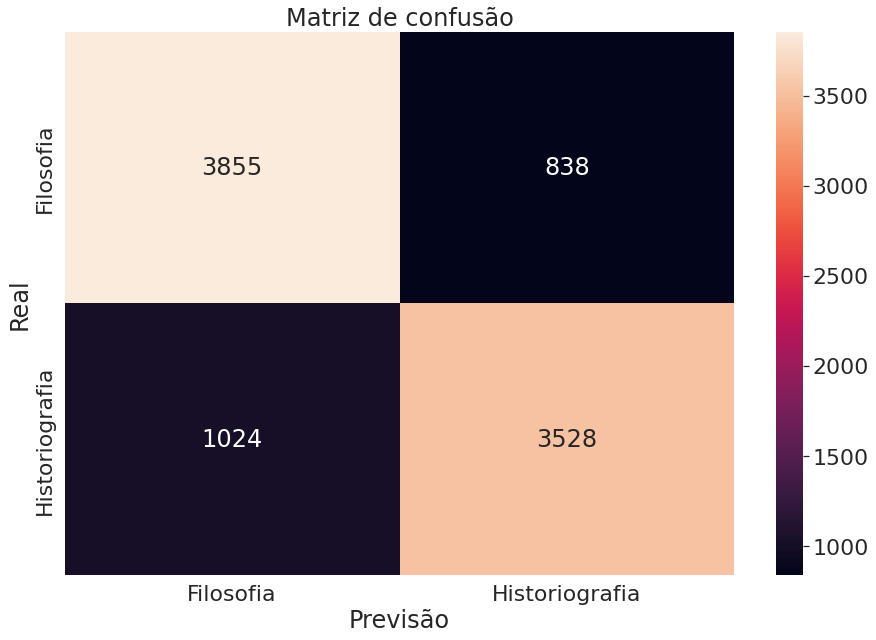
\includegraphics[width=.7\linewidth]{./figs/confusao.png}
	\end{center}
	\caption{Matriz de confusão para o modelo utilizado, métricas em~\autoref{tab:resumometrica}}\label{fig:confusao}
\end{figure}

\chapter{Discussão}

O próximo gráfico contém os coeficientes derivados pelo modelo para cada um dos verbos que pode reger um objeto oblíquo e oração infinitiva e que estão atestados no corpus de estudo.\footnote{Os coeficientes aqui são produzidos a partir da diferença entre as probabilidades de ocorrer em um texto filosófico e de ocorrer em um texto historiográfico. A classe de modelo Naïve-Bayes utilizada aqui estima a probabilidade de pertencer tanto ao gênero $g$ quanto ao gênero $\hat{g}$ (não-$g$), sendo assim necessário produzir um valor de diferença. A prática de contraste de coeficientes é comum na análise de modelos estatísticos bayesianos, cf.~\textcite{McElreath2020}.}
Valores positivos de coeficiente indicam que, estando esse verbo em um dado parágrafo, a probabilidade de que este parágrafo corresponda a um texto historiográfico sobe, e os valores negativos favorecem a hipótese de que o texto vem de um diálogo filosófico.
Por fim, as barras em verde marcam os verbos que denotam modalidade, as azuis verbos que denotam ações.
5
Os verbos com semântica modalizadora ocupam em sua maioria a região esquerda do gráfico, onde a presença de um item favorece a atribuição do parágrafo ao gênero filosófico, como previa a hipótese inicial. Apenas três verbos dessa classe possuem peso contrário, a saber sumferw, hyparxw e porw, sendo particularmente excepcional o caso do último.\footnote{A justificativa provavelmente está na baixíssima frequência de ocorrência deste verbo no corpus grego como um todo, com exceção apenas de Homero.}
Por outro lado, os verbos com semântica de `ordenar\slash{}aconselhar\slash{}etc.` estão concentrados na direita do gráfico, indicando a preferência por eles em textos historiográficos, embora a dispersão seja muito maior.

\begin{figure}[!ht]
	\begin{center}
		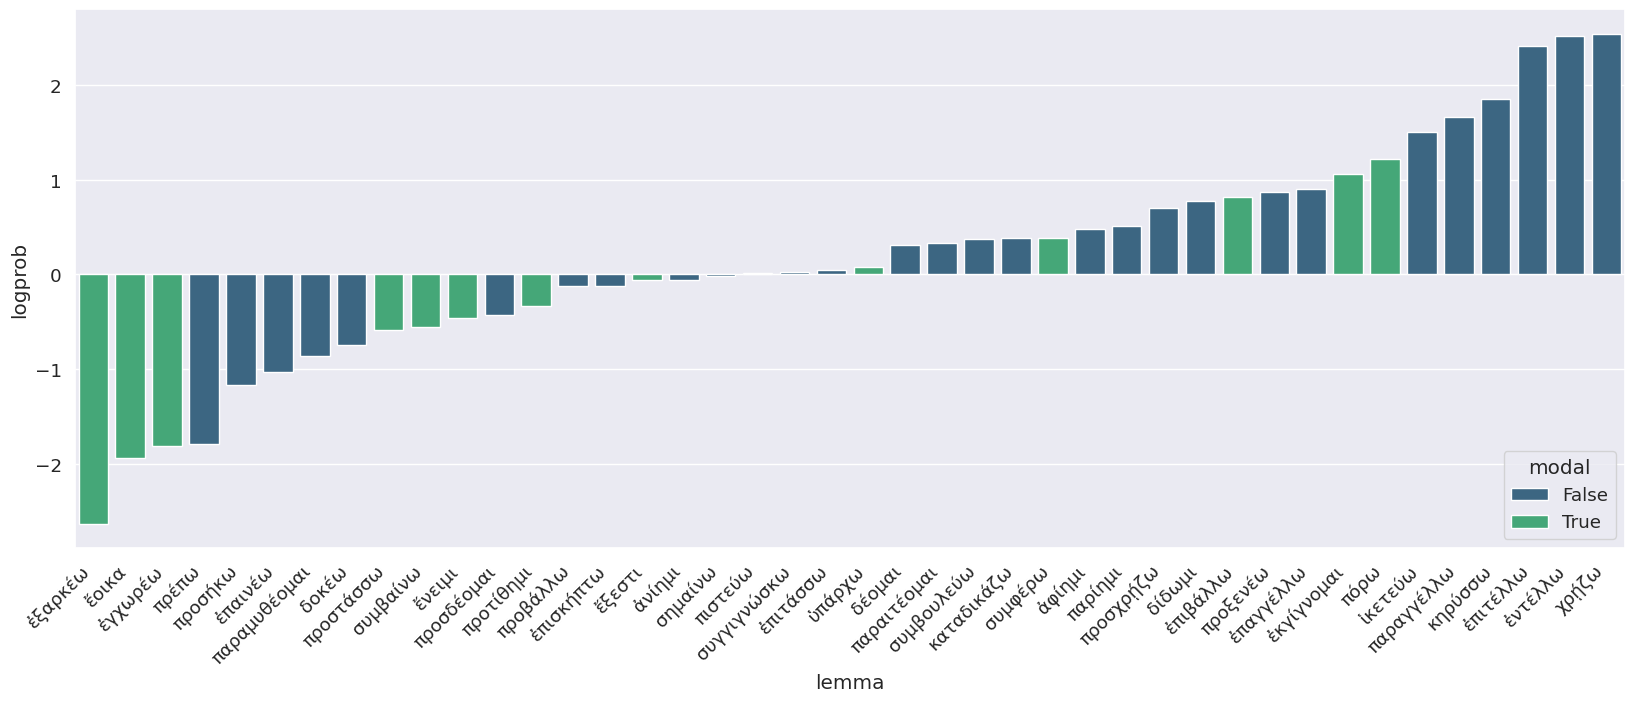
\includegraphics[width=1.0\linewidth]{./figs/diff2.png}
	\end{center}
\end{figure}

Uma palavra sobre as unidades pode ser importante: a escala logarítmica do eixo $y$ é utilizada em modelos porque computadores sofrem calculando probabilidades de 0 a 1 ou 0 a 100\% e ela é um tanto estranha de se interpretar. No exemplo acima, o verbo entellw tem um valor de aproximadamente $logit(2.5)$, o que equivale a algo na casa de $0.97$.
Isso é um valor \textbf{muito} alto.
Qualquer verbo cujo coeficiente ultrapasse a casa de $\pm logit(1.0)$ indica que a probabilidade condicional de que aquele verbo ocorra mais em um gênero textual do que outro é altíssima, ou ao menos que o modelo tem muita certeza disso e a faixa entre $logit(0.5)$ e $logit(0.75)$ não pode ser desprezada.
Assim, esse experimento oferece evidência de que:
\begin{compactenum}
\item a maioria dos verbos de interesse desta pesquisa com semântica modal estão associados ao gênero do diálogo filosófico grego;
\item alguns destes tem associação extremamente forte, servindo de ponto de contraste entre o gênero filosófico e historiográfico;
\item a maioria dos verbos de interesse que denotam ordens, conselhos etc.\ estão associados ao gênero de prosa filosófica; e
\item esta última classe de verbos é mais dispersa na escala do que a classe dos modalizadores.
\end{compactenum}

\printbibliography%

\end{document}
